\section{Dataset and Toolbox}
\subsection{MNIST}
Firstly, we want to check if the previously given algorithms work for a simple database. At the beginning of this internship, we had to rewrite a prototype with the full Sparse Coding pipeline (i.e. Algorithm 1 and 3 to 6). The goal here was to understand the underlying principles behind Sparse Coding.\\
To test this prototype and all our models, we have chosen the MNIST database, which is widely used in machine learning field. The MNIST database is composed of handwritten digits, available from Yann Lecun's website\footnote{\url{http://yann.lecun.com/exdb/mnist/index.html}}. MNIST has a training set of 50,000 examples and a test set of 10,000 examples (see figure \ref{fig:MNIST}). This is a subset of a larger dataset: NIST. \\
The digits have been size-normalized and centered in a fixed size of $28 \times 28$ pixels.\\
Generally having a model working on MNIST  is the first step before to test this model on other types of signal, such as speech.\\ 
\begin{mdframed}
\begin{center}
\textbf{That's why during this internship, we focused mainly on this dataset to test our models and the power of extracting discriminant features of Sparse Coding and Autoencoders and not directly on Speech.} 
\end{center}
\end{mdframed}

%One way to evaluate the quality of our results is to compare the original data vs the reconstructed ones. 
\begin{figure}[h]
 \centering
 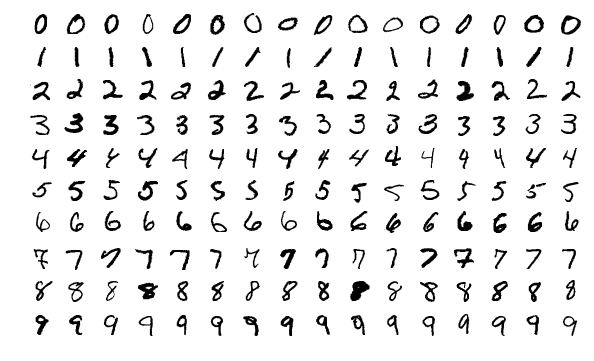
\includegraphics[scale=0.4]{MnistExamples.png}
 % MnistExamples.png: 594x361 px, 72dpi, 20.96x12.74 cm, bb=0 0 594 361
 \caption{Example of MNIST's handwritten digits}
  \label{fig:MNIST}
\end{figure}

The prototype, written in Python 3.6, computes Sparse Coding on a subset of the MNIST dataset to save time. This prototype is available on our GitHub repository \footnote{\url{https://github.com/Usanter/SparseCoding}} under the name: \texttt{SparseCoding.py}. \\
However, this prototype is not capable of training on all MNIST dataset, as we only used simple, non-optimized algorithms. In order to use the entire MNIST dataset, we used a toolbox called SPAMS that already includes some optimized algorithms for Sparse Coding.\\
\subsubsection{SPAMS}
SPAMS\footnote{\url{http://spams-devel.gforge.inria.fr/}}(\textbf{SPA}rse \textbf{M}odeling \textbf{S}oftware) is an optimization toolbox for solving various sparse estimation problems.
\begin{itemize}
 \item Dictionary learning and matrix factorization (NMF, sparse PCA, ...)
 \item Solving sparse decomposition problems with LARS, coordinate descent, OMP, SOMP, proximal methods
 \item Solving structured sparse decomposition problems (l1/l2, l1/linf, sparse group lasso, tree-structured regularization, structured sparsity with overlapping groups,...).
\end{itemize}
It is developed and maintained by J. Mairal (Inria), and contains sparse estimation methods resulting from collaborations with: F. Bach, J. Ponce, G. Sapiro, R. Jenatton and G. Obozinski, \dots\\
%You can find my code of Sparse Coding/Dictionary Learning on MNIST using SPAMS toolbox on my GitHub \texttt{test\_spams.py}.\\
\newpage
\section{Experimentation details}
\subsection{Application of traditional Coding on MNIST}

Here we use SPAMS toolbox, with algorithm 2 as Sparse Coding step and algorithm 6 for dictionary learning on the MNIST dataset. The choice of lambda (which influence the importance of the sparse term in the optimization) is given by  \cite{Mairal:2009:ODL:1553374.1553463} such that : $\lambda = \frac{1.2}{\sqrt{m}}$. \\
\begin{figure}[h]
 \centering
 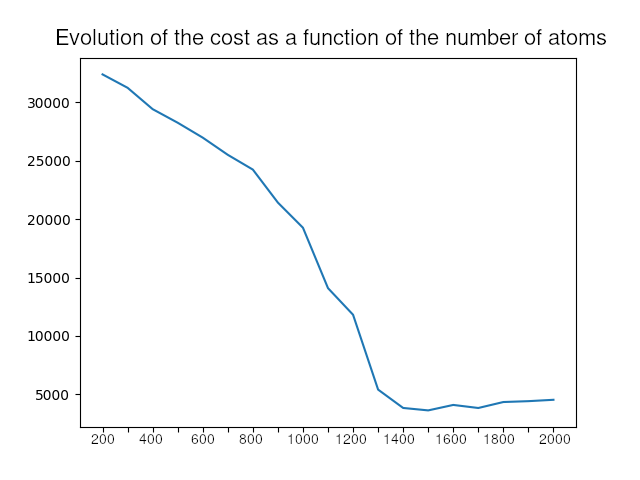
\includegraphics[scale=0.6]{Cost.png}
 % Cost.png: 640x480 px, 100dpi, 16.26x12.19 cm, bb=0 0 461 346
 \caption{Cost's evolution depends on the number of atoms in the dictionary}
 \label{fig:CostEvolution}
\end{figure}
\vspace{0.2cm}
Traditionally, during the learning of an overcomplete (or redundant) dictionary, the number of atoms $k$ so that $k \geq 2$ $*$ Signal's size.\\
All samples in the MNIST database have a size of 784 ( $28  \times 28$). Then, we compute for different values of k the cost function. We have obtained the cost function evolution. As expected the minimum of this cost function is reached when the number of atoms is more than 1400 atoms (see figure \ref{fig:CostEvolution}). This confirms the traditional assumption of the number of chosen atoms.
\begin{figure}[h]
 \centering
 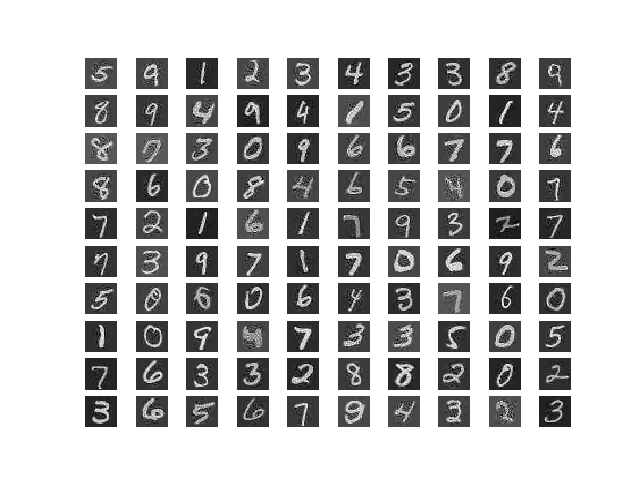
\includegraphics[scale=0.7]{D.png}
 % D.png: 640x480 px, 100dpi, 16.26x12.19 cm, bb=0 0 461 346
 \caption{Some of the 1400 atoms in the dictionary}
 \label{fig:D_1400k}
\end{figure}

\begin{figure}[h]
 \centering
 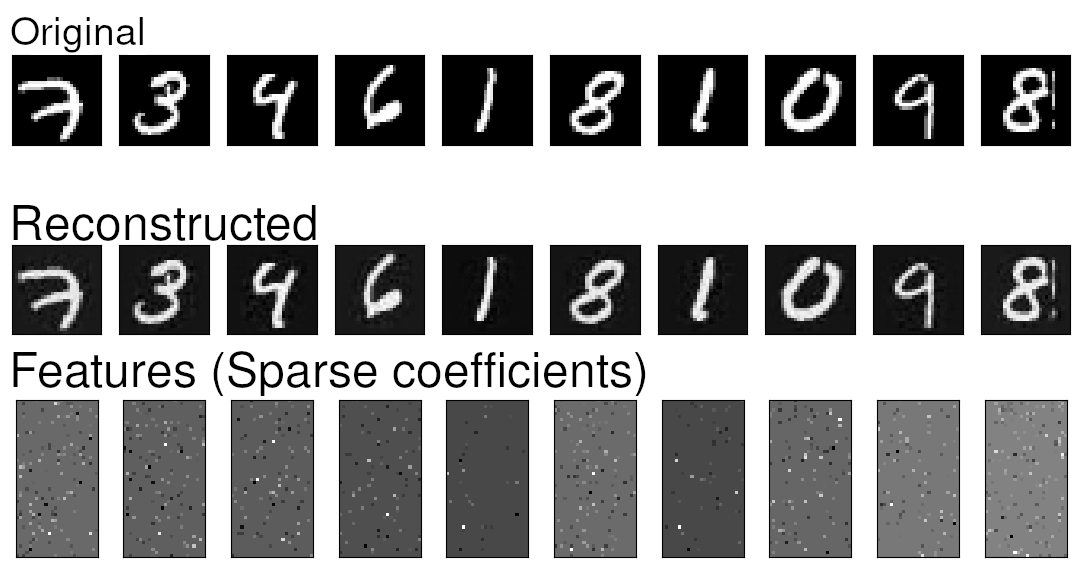
\includegraphics[scale=0.5]{normrecons.png}
 % normrecons.png: 1092x387 px, 100dpi, 27.74x9.83 cm, bb=0 0 786 279
 \caption{Reconstruction using $D \gamma$ and $\gamma$}
 \label{fig:Recons}
\end{figure}
The results obtained show that the handwritten numbers have a similar structure (for the same handwritten number).Most of the atoms in the dictionary (figure \ref{fig:D_1400k})  directly resemble a handwritten digit (with little noise for some of them). Notice that the reconstruction looks good as shown in figure \ref{fig:Recons} .
% \subsection{Application on Hade/Hide dataset}
% In HideHade dataset, all data doesn't have the same length. The smallest is approximatively 0.3 seconds whereas the longest one is approximatively 0.9 seconds. Due to this, we can use directly on the signal our Sparse Coding algorithm. To solve this problem we use a sliding window of 512 samples and with a overlapping of 256 samples (see examples figure \ref{fig:SlidingWin}).
% \begin{figure}[h]
%  \centering
%  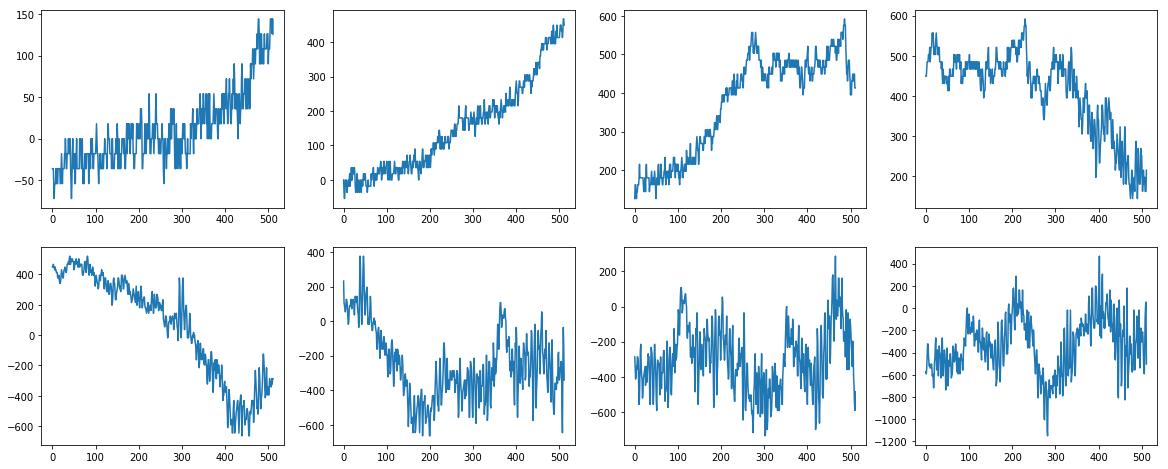
\includegraphics[scale=0.3]{slidingwindows.png}
%  % slidingwindows.png: 2842x1122 px, 72dpi, 100.28x39.59 cm, bb=0 0 2843 1122
%  \caption{Example of samples extract by sliding window}
%  \label{fig:SlidingWin}
% \end{figure}
% \begin{figure}[h]
%  \centering
%  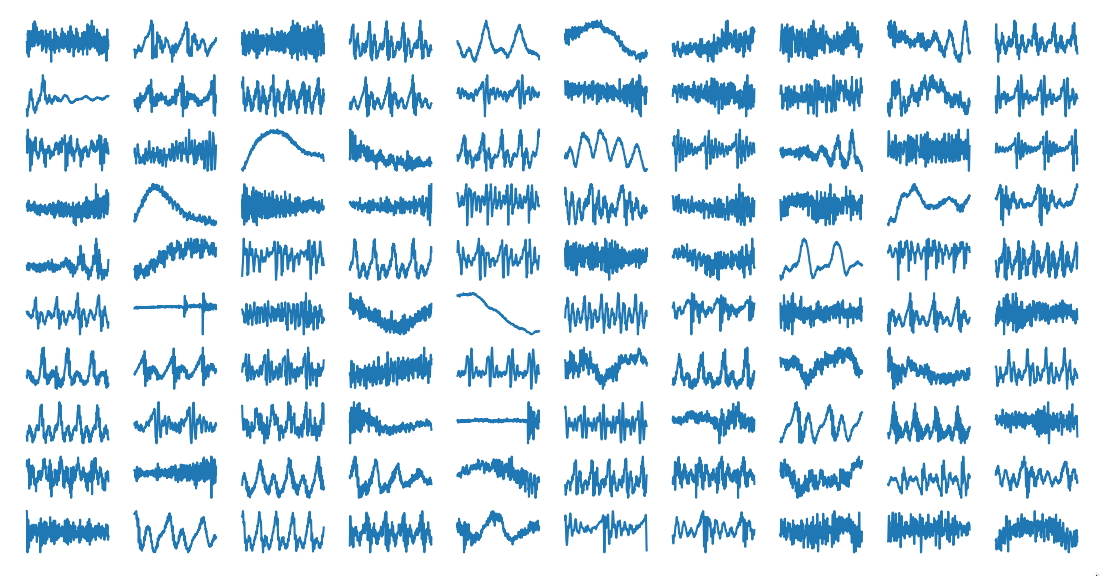
\includegraphics[scale=0.43]{DHH.png}
%  % DHH.png: 1105x576 px, 96dpi, 29.23x15.24 cm, bb=0 0 829 432
%  \caption{Example of atoms in the dictionary}
%  \label{fig:Dhh}
% \end{figure}
% \begin{figure}[h]
%  \centering
%  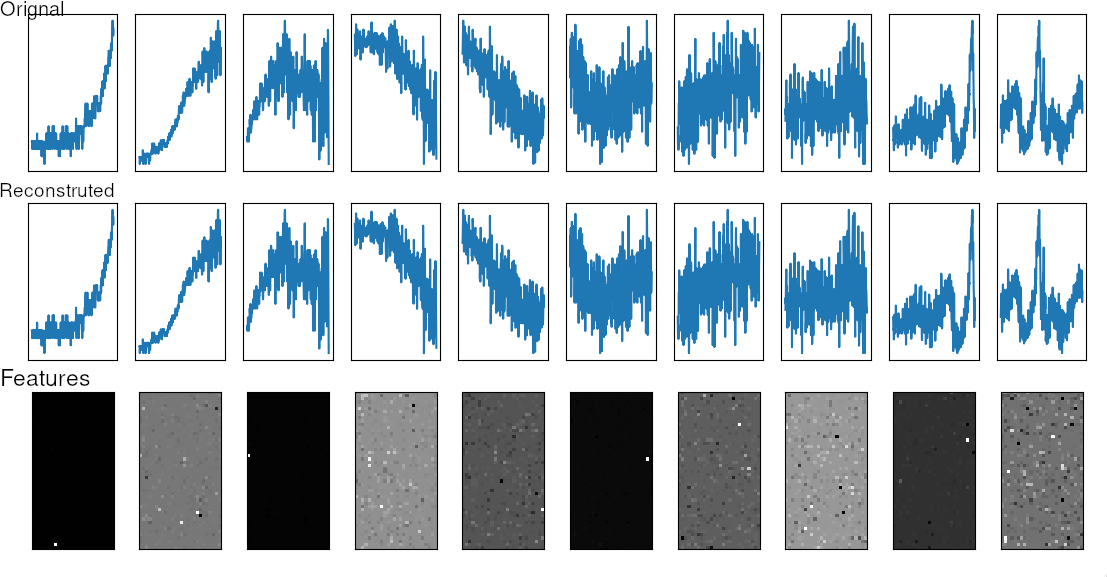
\includegraphics[scale=1.5]{SCHH.png}
%  % SCHH.png: 1107x577 px, 300dpi, 9.37x4.89 cm, bb=0 0 266 138
%  \caption{Examples of reconstruction and associated features}
%  \label{fig:SCHH}
% \end{figure}
% 

\subsection{Classification for traditional Sparse Coding}
In the internship's context, we always tried two different classifiers on our data: SVM and K-means. 
SVM is a supervised classifier, while K-mean is an unsupervised one. The goal here is to highlight the discriminatory power of Sparse coding through a supervised and unsupervised manner.\\
For the traditional Sparse coding, the obtained accuracies are:
\begin{itemize}
 \item SVM accuracy: 0.90 
 \item K-means accuracy: 0.1319
\end{itemize}
As we can see, we have good results for the SVM classifier but very bad results for the K-means, if we take the sparse coefficients in an unsupervised manner, the sparse coefficients are not discriminative.\\

Whereas the previous tests seem to have a good result in reconstruction, one question appears: \\

\begin{center}
\fbox{\begin{varwidth}{\textwidth}
\centering
\textit{What makes us confident about the fact that two signals with the same label (for example two handwritten number 3 ) have close sparse coefficients representation $\gamma$ after the Sparse Coding step?}
\end{varwidth}}
%\fbox{\textbf{Definition:} \\Sparse:
%\textit{ Occurring at widely spaced intervals, not thick or dense.}}
\end{center}
 In fact, nothing guarantees this assumption.  The signal processing community asked themselves about this question. To ensure to have discriminative sparse code representation they created an extension of traditional Sparse Coding called Discriminative Sparse coding.
% Put here a table with results with SVM and Kmeans
% \paragraph{Test 1}
% In the first test, I used 256 atoms, 2 000 iterations and $\lambda$ = 0.015 to learn the dictionary and the sparse coefficients. 
% w\begin{figure}[h]
%  \centering
%  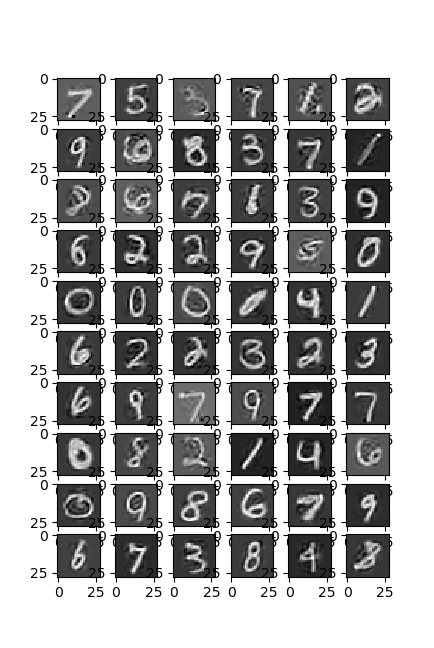
\includegraphics[scale=0.82]{../Results/SPAMS_X_ALL_K256/D.png}
%  % D.png: 434x648 px, 100dpi, 11.02x16.46 cm, bb=0 0 312 467
%  \caption{Few atoms of D}
% \end{figure}
% 
%  \begin{figure}[h]
%  \begin{subfigure}{.5\textwidth}
%  \centering
%  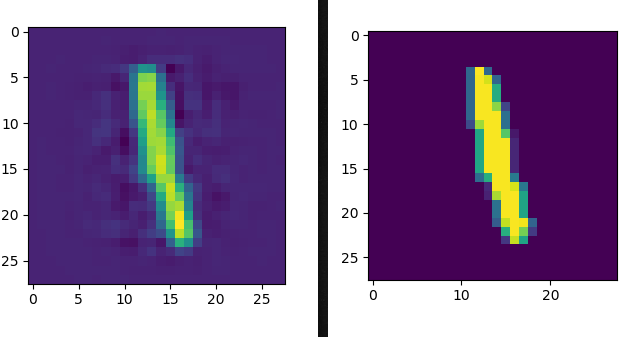
\includegraphics[scale=0.35]{../Results/SPAMS_X_ALL_K256/recons_1.png}
%   \caption{Reconstructed 1 vs Original 1}
%  % module-capteur-laser.jpg: 600x600 px, 72dpi, 21.17x21.17 cm, bb=0 0 600 600
%  \end{subfigure}%
%   \begin{subfigure}{.3\textwidth}
%  \centering
%  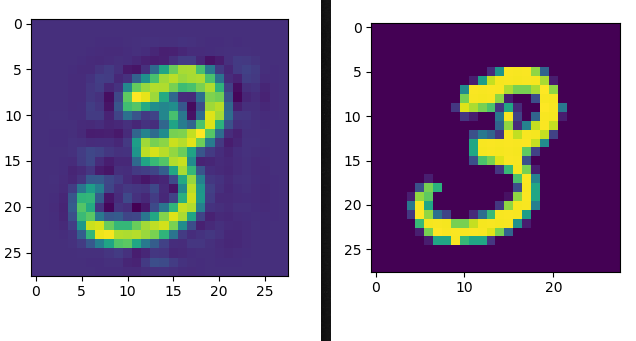
\includegraphics[scale=0.35]{../Results/SPAMS_X_ALL_K256/recons_3.png}
%  % module-capteur-laser.jpg: 600x600 px, 72dpi, 21.17x21.17 cm, bb=0 0 600 600
%   \caption{Reconstructed 3 vs Original 3}
% 
%  \end{subfigure}%
% \end{figure}
% 
% \newpage
% 
% \paragraph{Test 2}In the second test I used 1024 atoms, 1 000 iterations and $\lambda = \frac{1.2}{\sqrt{m}}$ \cite{Mairal:2009:ODL:1553374.1553463} \textit{(In my case $\approx 0.0042857$)}.
% \begin{figure}[h]
%  \centering
%  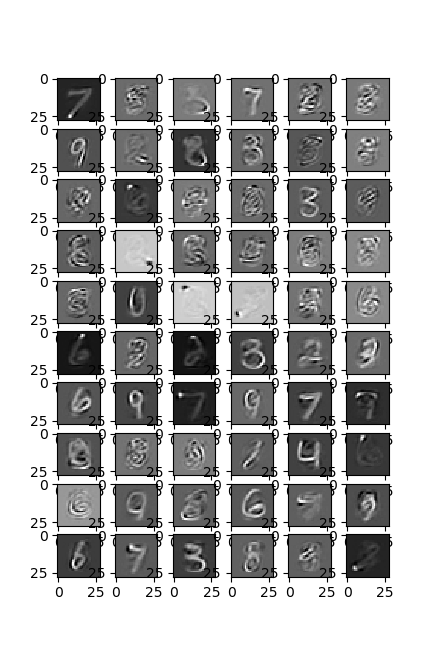
\includegraphics[scale=0.82]{../Results/SPAMS_X_ALL_K1024/D.png}
%  % D.png: 1873x1022 px, 100dpi, 47.57x25.96 cm, bb=0 0 1349 736
%  \caption{Few atoms of D}
% \end{figure}
%  \begin{figure}[h]
%  \begin{subfigure}{.5\textwidth}
%  \centering
%  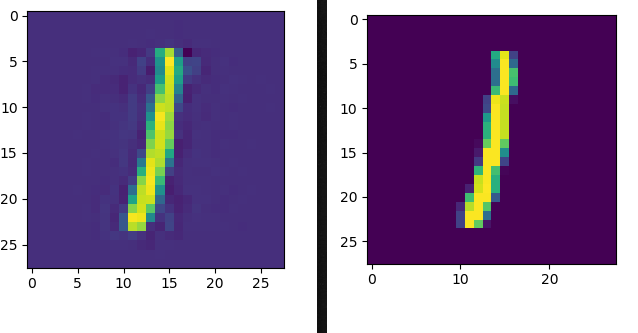
\includegraphics[scale=0.4]{../Results/SPAMS_X_ALL_K1024/lambdaopti_recons1.png}
%   \caption{Reconstructed 1 vs Original 1}
%  % module-capteur-laser.jpg: 600x600 px, 72dpi, 21.17x21.17 cm, bb=0 0 600 600
%  \end{subfigure}%
%   \begin{subfigure}{.3\textwidth}
%  \centering
%  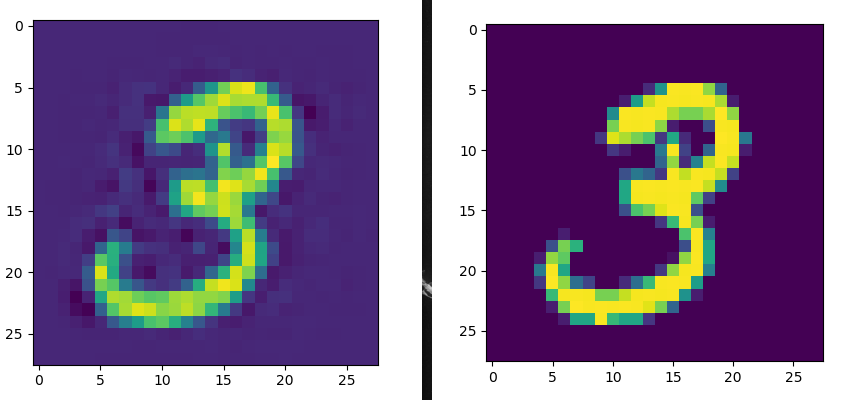
\includegraphics[scale=0.29]{../Results/SPAMS_X_ALL_K1024/lambdaopti_recons3.png}
%  % module-capteur-laser.jpg: 600x600 px, 72dpi, 21.17x21.17 cm, bb=0 0 600 600
%   \caption{Reconstructed 3 vs Original 3}
% 
%  \end{subfigure}%
% \end{figure}
% \newpage
% \paragraph{Test 3} In the third test I used 1024 atoms, 1 000 iterations and $\lambda = 5$.
% \begin{figure}[h]
%  \centering
%  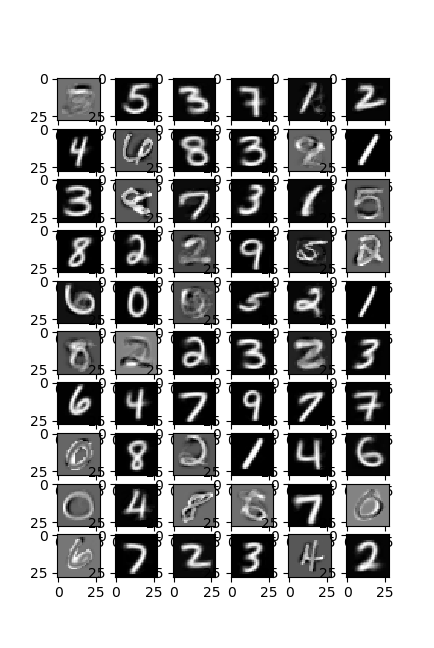
\includegraphics[scale=0.82]{../Results/SPAMS_X_ALL_K1024/D_lambdagrand.png}
%  % D_lambdagrand.png: 936x994 px, 100dpi, 23.77x25.25 cm, bb=0 0 674 716
%  \caption{Few atoms of D}
% \end{figure}
% 
%  \begin{figure}[h]
%  \begin{subfigure}{.5\textwidth}
%  \centering
%  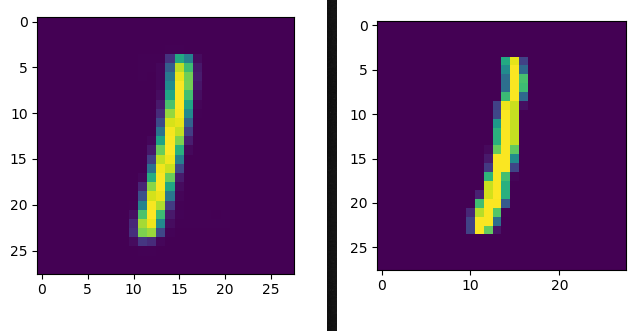
\includegraphics[scale=0.4]{../Results/SPAMS_X_ALL_K1024/lambdagrand_recons1.png}
%   \caption{Reconstructed 1 vs Original 1}
%  % module-capteur-laser.jpg: 600x600 px, 72dpi, 21.17x21.17 cm, bb=0 0 600 600
%  \end{subfigure}%
%   \begin{subfigure}{.3\textwidth}
%  \centering
%  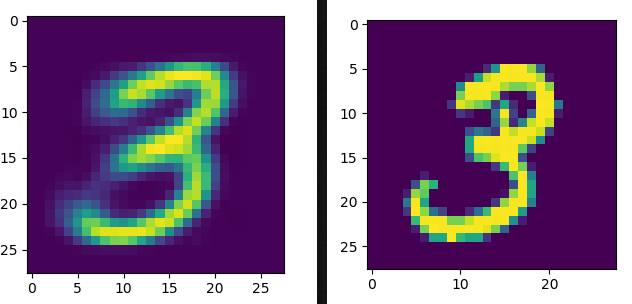
\includegraphics[scale=0.39]{../Results/SPAMS_X_ALL_K1024/lambdagrand_recons3.png}
%  % module-capteur-laser.jpg: 600x600 px, 72dpi, 21.17x21.17 cm, bb=0 0 600 600
%   \caption{Reconstructed 3 vs Original 3}
% 
%  \end{subfigure}%
% \end{figure}
% 
% \newpage
% \paragraph{Test 4} In the fourth test I used 2048 atoms, 1 000 iterations and $\lambda = \frac{1.2}{\sqrt{m}}$
% \begin{figure}[h]
%  \centering
%  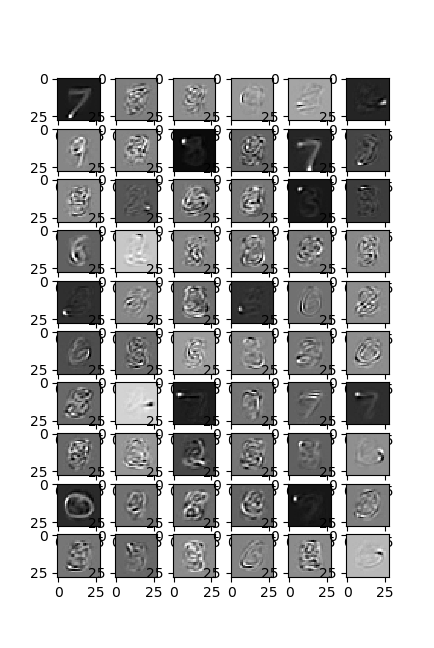
\includegraphics[scale=0.82]{../Results/SPAMS_X_ALL_K_2048/D_K2048.png}
%  % D_K2048.png: 936x994 px, 100dpi, 23.77x25.25 cm, bb=0 0 674 716
%  \caption{Few atoms of D}
%  \end{figure}
%  
%   \begin{figure}[h]
%  \begin{subfigure}{.5\textwidth}
%  \centering
%  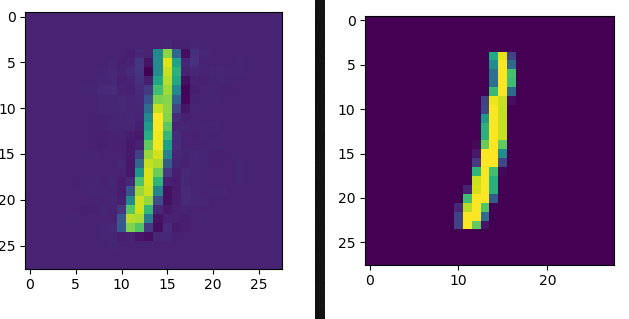
\includegraphics[scale=0.4]{../Results/SPAMS_X_ALL_K_2048/recons1.png}
%   \caption{Reconstructed 1 vs Original 1}
%  % module-capteur-laser.jpg: 600x600 px, 72dpi, 21.17x21.17 cm, bb=0 0 600 600
%  \end{subfigure}%
%   \begin{subfigure}{.3\textwidth}
%  \centering
%  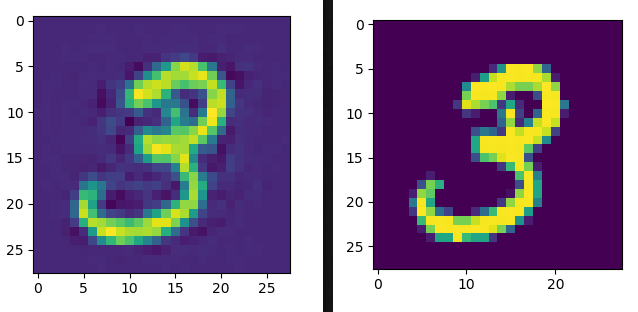
\includegraphics[scale=0.39]{../Results/SPAMS_X_ALL_K_2048/recons3.png}
%  % module-capteur-laser.jpg: 600x600 px, 72dpi, 21.17x21.17 cm, bb=0 0 600 600
%   \caption{Reconstructed 3 vs Original 3}
% 
%  \end{subfigure}%
% \end{figure}
% 
% \newpage
